This section first introduces notation, 
definitions, and the classification task.
We then describe the relevant technical details
of sparse SA prevalent in the GT literature,
and review the \textsc{GCN-SA} architecture.
Finally, we describe how sparse SA 
is integrated with \textsc{GCN-SA}.

\subsection{Problem Formulation}
Notation will mostly follow \citet{jiang2024self}
and should be rather unsurprising.
Let $ G = (V, E) $ be an undirected graph,
where $ V $ and $ E $ are the sets of nodes
and edges respectively.
We define $ n = |V| $ to be the number of nodes
in the graph.
Let $ \mathbf{A} \in \mathbb{R}^{n \times n} $
be the (symmetric) adjacency matrix of $ G $,
where $ A_{ij} 
=\mathbbm{1} \left\{ e_{ij} \in E \right\} $.
Denote 
$ \mathbf{X} = 
\begin{bmatrix}
  \mathbf{x}_1& \cdots & \mathbf{x}_n
\end{bmatrix}^\top
\in \mathbb{R}^{n\times d} $
as our feature matrix,
where $ \mathbf{x}_i \in \mathbb{R}^d$
corresponds to the features of node $ v_i \in V $.
Finally, for a set of classes 
$ [c] = \left\{ 1, \cdots, c \right\} $
and a subset of labelled nodes
$ V_{\text{lab}} \subset V $,
$ \mathbf{y}_{\text{lab}} \in [c]^{|V_{\text{lab}}|} $
are the corresponding labels.

Our inference task is to predict the labels of the unlabeled nodes
given positional and semantic information
($\mathbf{A}$ and $\mathbf{X}$ respectively).
More formally,
find the posterior distribution
$ 
    \mathbf{y}
    \mid \mathbf{X}, \mathbf{A}, \mathbf{y}_{\text{lab}}
$
for completed label vector $ \mathbf{y} \subset [c]^n $.

Another important definition to consider is the \emph{homophily ratio}
of a graph:
\begin{definition}[Homophily Ratio]
  For graph $ G = (V, E) $,
  the homophily ratio $ h $ is 
  \begin{flalign*}
    h = \frac{|\{(v_i,v_j) \in E\colon y_i = y_j\}|}{|E|}.
  \end{flalign*}
\end{definition}

As $h \to 1 $, 
$ G $ becomes completely homophilous (high-homophily)
and as $h \to 0 $, 
$ G $ becomes completely heterophilous (low-homophily) 
\citep{zhu2020beyond}.
For our experiments, we note the homophily ratio
corresponding to each graph.


\subsection{(Sparse) Self-Attention}
Per \citet{zaheer2020big},
recall the definition for a \emph{generalized attention mechanism}
and a \emph{sparse attention mechanism}.

\begin{definition}[Generalized Attention Mechanism]
  $ \textsc{Attn}_D\colon \mathbb{R}^{n\times d}
  \to \mathbb{R}^{n\times n} $
  is a generalized attention mechanism 
  if it can be characterized by a digraph 
  $ D = ([n] = \left\{ 1, \cdots, n \right\}, E_D) $
  where $ e_{ij} \in E_D $ if $ v_i $ attends $ v_j $.
  The attention scores for $ \mathbf{x}_i $ with $ H $ heads
  is
  \begin{flalign*}
    \textsc{Attn}_D(\mathbf{X})_{i}
    &= \mathbf{x}_i
    + \sum_{h=1}^{H} \textrm{softmax} \left(
      Q_h(\mathbf{x}_i)
      K_h(\mathbf{X}_{N(i)})^\top
    \right)
    \cdot V_h(\mathbf{X}_{N(i)})
  \end{flalign*}

  where $ N(i) = \left\{ j\colon e_{ij} \in E_D \right\}$
  denotes the nodes that $ i $ attends to,
  $ \mathbf{X}_{N(i)} $ the submatrix
  of $ \mathbf{X} $ with columns in $ N(i) $,
  $ Q_h, K_h \colon \mathbb{R}^d \to \mathbb{R}^m $
  the query and key functions,
  and 
  $ V_h\colon \mathbb{R}^d \to \mathbb{R}^d $
  the value function.
\end{definition}

\begin{definition}[Sparse Attention Mechanism]
  We say the attention mechanism
  $ \textsc{Attn}_D $ is \emph{sparse} if
  $ |E_D| \in o(n^2) $,
  and more specifically $ \textsc{Attn}_D $
  is linear if $ |E_D| \in \mathcal{O}(n) $.
\end{definition}

Approaches to find $ D $ satisfying sparsity
typically follow graph-theoretic approaches
(e.g. expander graphs for expander attention
in \textsc{Exphormer}),
yielding desirable properties.
Most importantly,
sparse SA mechanisms can be universal approximators,
preserving the properties of full quadratic models
\citep{zaheer2020big}.
In practice, sparse SA has performed comparably 
or even better than full SA
on a wide array of tasks \citep{shirzad2023exphormer}.

With this in mind,
we suspect that sparse attention may improve 
the overall runtime of \textsc{GCN-SA}
with minimal performance hit.


\subsection{GCN-SA}
The high-level motivation of GCN-SA
is to combine three sources 
of information for learning by the downstream GCN:
node feature information,
short-range, and long range structural information
We focus on the long-range structure learning by
\textsc{GCN-SA}'s utilization of SA
with \emph{reconnected adjacency matrix generation}.

\begin{figure}
  \centering
  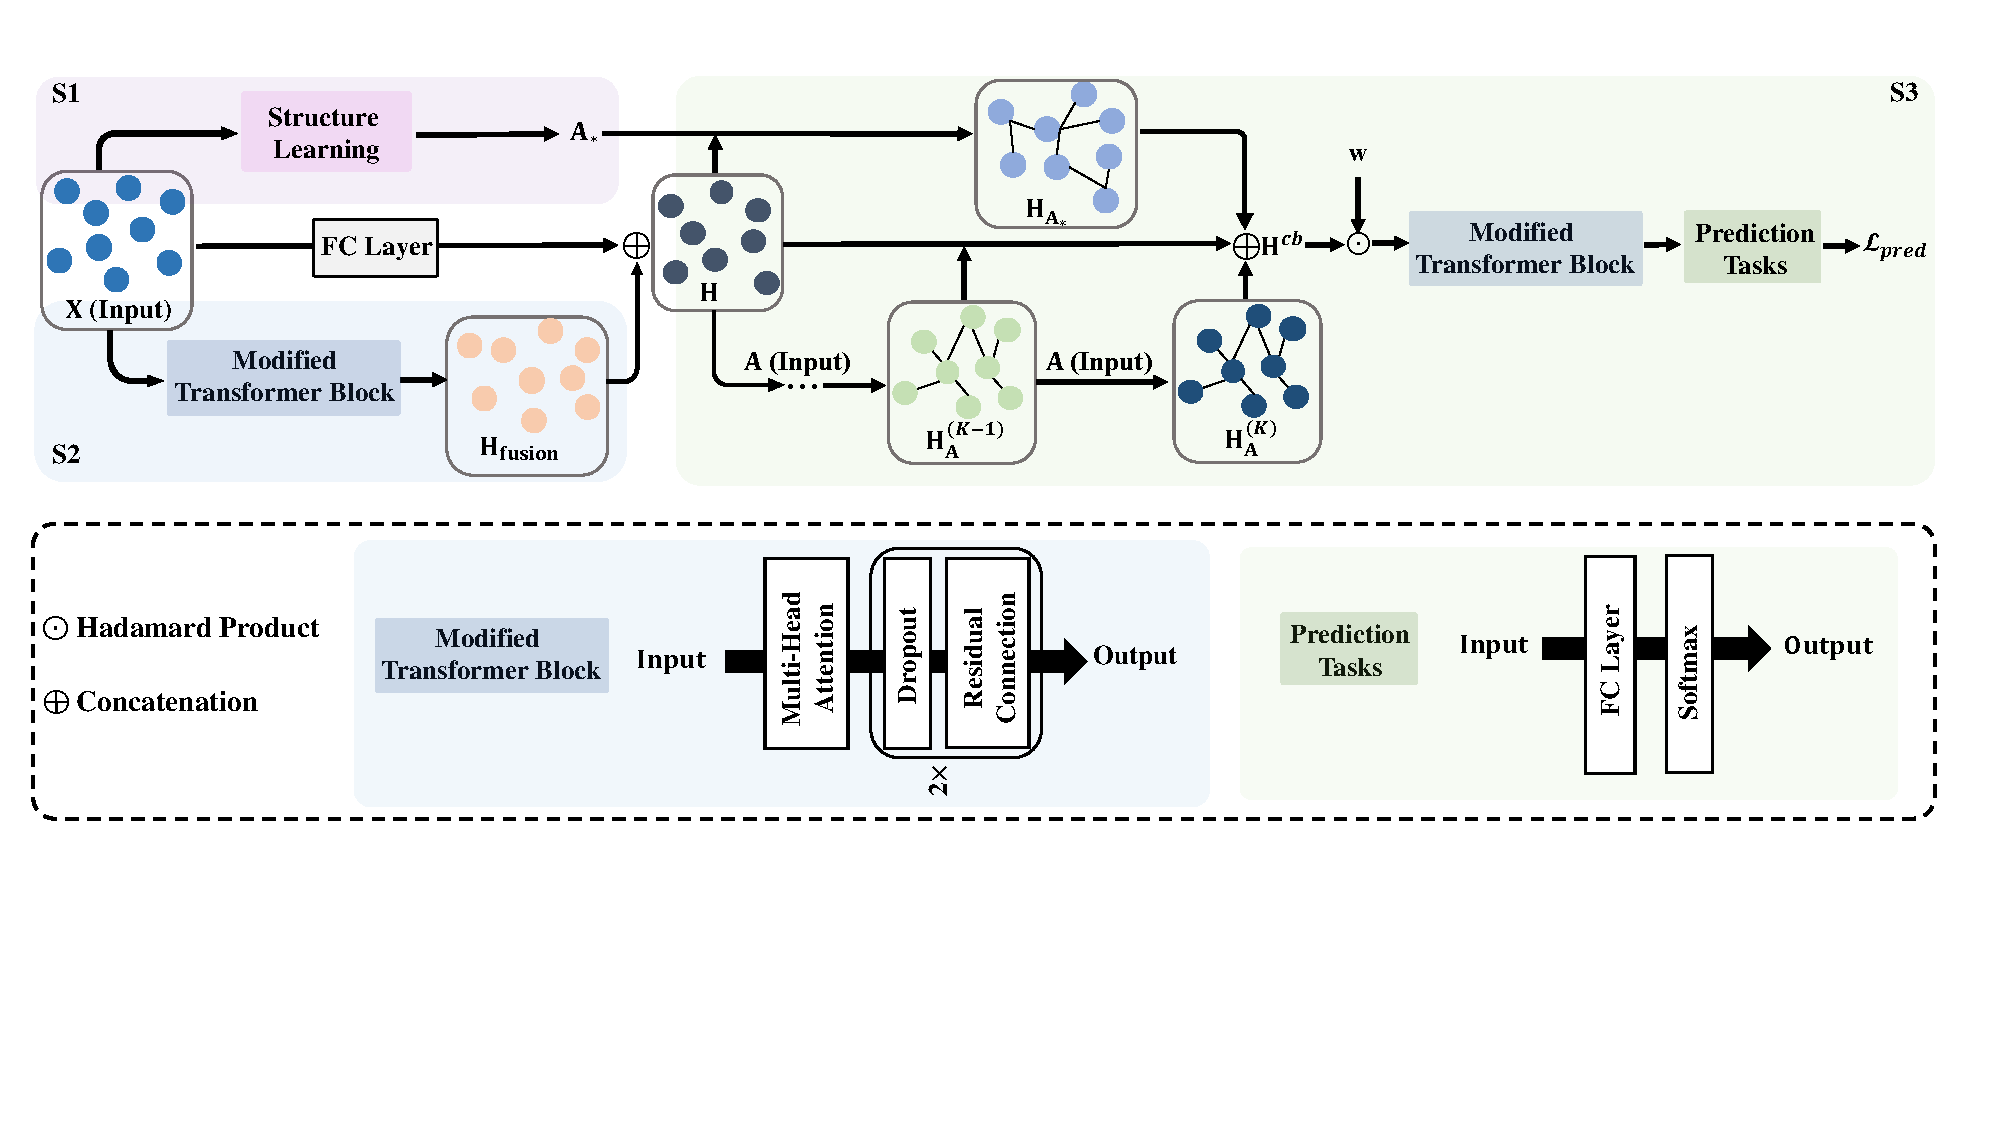
\includegraphics[page=1, width=\linewidth]{src/flowchart.pdf}
  \label{fig:flowchart}
  \caption{\textsc{GCN-SA} architecture
  \citep{jiang2024self}.}
\end{figure}

% \subsubsection{Reconnected Adjacency Matrix}

The motivation for learning a reconnected adjacency matrix
is to represent long-range connections between nodes.
An attention score matrix 
$ \mathbf{S} \in \mathbb{R}^{n\times n}$
is formed to generate a sparse reconnected adjacency matrix
$ \mathbf{A}^* \in \mathbb{R}^{n\times n}$
via $ H $-headed multi-head self-attention (MHSA):
\begin{flalign}
  \mathbf{S}
  &= \frac{1}{H} \sum_{h=1}^{H}
  \textrm{cosine}(\mathbf{X}\mathbf{W}_h^{Q}),
\end{flalign}

where $ \mathbf{W}_h^{Q} \in \mathbb{R}^{d\times p}  $
are learnable parameters corresponding to head
$ h = 1, \cdots, H $,
$ \textrm{cosine}\colon 
\mathbb{R}^{n \times p} \to [-1, 1]^{n \times n} $ 
the pairwise cosine similarity function for matrix
columns,
and $ \mathbf{S} \in [-1, 1]^{n \times n} $ the attention score matrix.
Once $ \mathbf{S} $ is obtained,
we construct the reconnected adjacency matrix
$ \mathbf{A}^* \in \left\{ 0, 1 \right\}^{n\times n} $
with a combined
$ k $NN and minimum-threshold approach:
\begin{flalign*}
  A^*_{ij} = \mathbbm{1} \left\{ 
    S_{ij} > \varepsilon \text{ or } S_{ij} \in R_i
  \right\}
\end{flalign*}

for hyperparameters $ \varepsilon, r $
and $ R_i $ denotes the $ r $ largest elements
of row $ S_{i\cdot} $.
A minor point is afterwards we set 
$ A^*_{ij} = \max \left\{ A^*_{ij}, A^*_{ji} \right\}$
to enforce symmetry.
The intention of this procedure 
is to ensure $ \mathbf{A}^* $ is \emph{sparse}
for better downstream performance \citep{jiang2024self}.
More specifically, each node attends to
$ \mathcal{O}(1) $ other nodes.
We touch on this in subsection 2.4.
For simplicity the authors denote
\begin{flalign*}
  \mathbf{A}^*
  &= \textrm{StructureLearning}(\mathbf{X}; \mathbf{W}^Q).
\end{flalign*}

parameterized by 
query parameters 
$ \mathbf{W}^Q = (
  \mathbf{W}^Q_1,
  \cdots, 
  \mathbf{W}^Q_H
) $.
Once $ \mathbf{A}^* $ is computed,
it is used downstream to compute
$ \mathbf{H}_{\mathbf{A}^*} $, 
representing aggregated long-range information:
\begin{flalign*}
  \mathbf{H}_{\mathbf{A}^{*}}
  = \mathbf{D}_*^{- \frac{1}{2}}
    \mathbf{A}^{*}
    \mathbf{D}_*^{- \frac{1}{2}}
    \mathbf{H}
\end{flalign*}

for $ \mathbf{D}_* = \text{diag}(\mathbf{A}^* \mathbf{1}_n) $ 
the degree matrix of $ \mathbf{A}^* $
and $ \mathbf{H} \in \mathbb{R}^{n \times q} $
representing node embeddings with hidden dimension $ q $.
% \mathbf{H}_\mathbf{A}^{*} 
% = \textrm{Fuse}(\mathbf{A}^{*}, \mathbf{H})
% \in \mathbb{R}^{n\times d}
% $. 
% Details on Fuse are included in the appendix.

% \subsubsection{Modified Transformer Block}

% Stages 2 and 3 of \textsc{GCN-SA} utilize a 
% transformer block:
% a fully-connected layer 
% followed by a self-attention layer.
% To mitigate overfitting
% (an issue prone to GCNs \citep{jiang2024self}),
% self-attention is followed by residual connection and dropout.
% The query parameters $ \mathbf{W}^Q $ are re-used
% in the transformer.
% We denote
% \begin{flalign*}
%   \mathbf{H} = \textrm{ModifiedTransformerBlock}(
%     \mathbf{X};
%     \mathbf{W}^Q,
%     \mathbf{W}^K,
%     \mathbf{W}^V,
%     \mathbf{W}^0
% )
% \end{flalign*}

% parameterized by the query, key, value,
% and fully-connected parameters.
% More detailed mathematical description
% can be seen is the appendix.

% \subsubsection{Feature Aggregation}

% Stepping back a little,
% GCN-SA utilize the reconnected adjacency
% matrix and the modified transformer blocks
% for feature aggregation in the following
% key sections of computation:
% \begin{enumerate}
%   \item Reconnected matrix formed from node features:
%     $ \mathbf{A}^* = \textrm{StructureLearning}(\mathbf{X}) $,
%   \item Feature embeddings 
%     $ \mathbf{H} \in \mathbb{R}^{n \times q} $ are formed 
%     from transformer block:
%     $ \mathbf{H} 
%     = \textrm{ModifiedTransformerBlock}(\mathbf{X}) $
%   \item $ \mathbf{H}_\mathbf{A}^{(k-1)},
%     \mathbf{H}_\mathbf{A}^{(k)} \in \mathbb{R}^{n \times q}$,
%     representing short-range structural information of $ G $,
%     are computed as:
%     $ \mathbf{H}_\mathbf{A}^{(k)} 
%     = \textrm{Fuse}(\mathbf{A}, \mathbf{H}_\mathbf{A}^{(k)}) $
%     for hyperparameter $ k $
%     and feature fusion function $ \textrm{Fuse} $.
%     Details on Fuse are included in the appendix.
%   \item $ \mathbf{H}^{cb} $, representing the combined information
%     of node features, short-range, and long-range structural
%     information,
%     is formed by concatenation:
%     \begin{flalign*}
%       \mathbf{H}^{cb} = \begin{bmatrix}
%         \mathbf{H}_\mathbf{A}^{(k-1)} &  
%         \mathbf{H}_\mathbf{A}^{(k)} &
%         \mathbf{H}_\mathbf{A}^{*} &
%         \mathbf{H}
%       \end{bmatrix}
%       \in \mathbb{R}^{n \times 4q}.
%     \end{flalign*}
% \end{enumerate}


\subsection{Modifying GCN-SA with Sparse SA}
This section describes the central contribution of the paper:
replacing the expensive SA computations in \textsc{GCN-SA}
with sparse equivalents.

Observe that the runtime of 
$ \text{StructureLearning}$ 
is $ \mathcal{O}(n^2d) $ due to the full SA mechanism.
We can reduce the runtime from quadratic (in $ n $)
to linear by replacing $ \text{StructureLearning} $
with a sparse SA mechanism.

\text{StructureLearning} will have 
better runtime complexity.
For instance,
\textsc{Exphormer}'s
expander attention and global attention
yield a runtime of 
$\mathcal{O}(nd)$
(we exclude \textsc{Exphormer}'s local attention
as we are only concerned with long-range dependencies).

Downstream in the model, $ \mathbf{A}^* $
is only used once more to compute $ \mathbf{H}_{A^*} $
As $ \mathbf{A}^* $ computed with the full SA
and $ k $NN + minimum-threshold approach is sparse
($\mathcal{O}(1)$ non-zero entries per row),
the computation of $ \mathbf{H}_{A^*} $
already occurs in $ \mathcal{O}(nq) $
and remains unchanged with our modified architecture.

